\documentclass[11pt]{article} % use larger type; default would be 10pt

\usepackage{tikz}
\usetikzlibrary{calc}

        \newcommand\degree[0]{^{\circ}}

\title{Play with TikZ}
\author{Just Us}
%\date{} % Activate to display a given date or no date (if empty),
         % otherwise the current date is printed 

\begin{document}
\maketitle

\section{Grid}

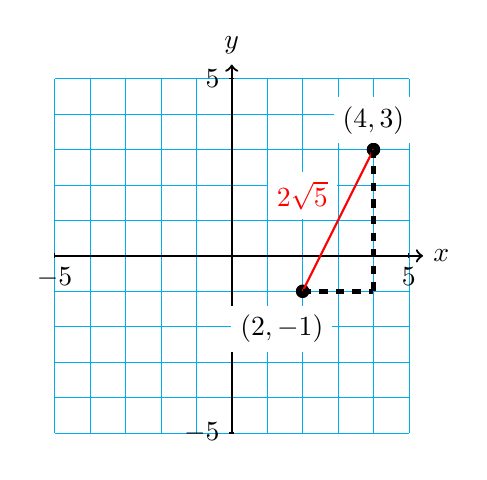
\begin{tikzpicture}[scale=.45]


\draw[step=1cm,cyan,very thin] (-5,-5) grid (5,5);
\draw[thick,->] (-5,0) -- (5.4,0) node[anchor=west] {$x$};
\draw[thick,->] (0,-5) -- (0,5.4) node[anchor=south] {$y$};
`
\foreach \x in {-5,5}
    \draw (\x cm,2pt) -- (\x cm,-2pt) node[anchor=north] {$\x$};
\foreach \y in {-5,5}
    \draw (2pt,\y cm) -- (-2pt,\y cm) node[anchor=east] {$\y$};


\coordinate (A) at (2,-1);
\coordinate (B) at (4,-1);
\coordinate (C) at (4,3);

\filldraw[black] (A) circle (5pt) node[anchor=north east,xshift=11,yshift=-5,fill=white] {$(2,-1)$};
\filldraw[black] (C) circle (5pt) node[anchor=south ,yshift=2,fill=white] {$(4,3)$};

\draw[red, thick] (A)--(C) node[above left, midway,fill=white] {$2\sqrt{5}$};
\draw[black, ultra thick, dashed] (A)--(B) ;
\draw[black, ultra thick, dashed] (C)--(B) ;


\end{tikzpicture}
\newline


circle
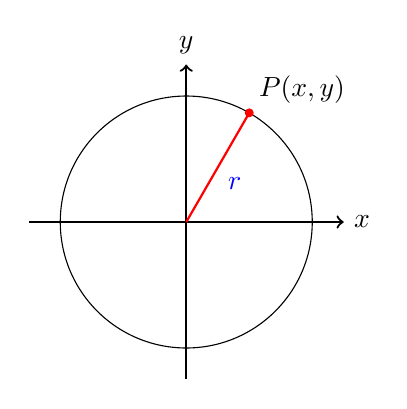
\begin{tikzpicture}

\coordinate(O) at (0,0);
\coordinate (A) at (0.8,1.386 );

\draw (0,0) circle (1.6);

\draw[thick,->] (-2,0) -- (2,0) node[anchor=west] {$x$};
\draw[thick,->] (0,-2) -- (0,2) node[anchor=south] {$y$};

\filldraw[red] (A) circle (1.4pt) node[anchor=south west, xshift=0, yshift=0]{\color{black}$P(x,y)$};

\draw[red, thick] (O) -- (A) node[below right, midway]{\color{blue}$r$};

\end{tikzpicture}
\newline


exam1-3-2
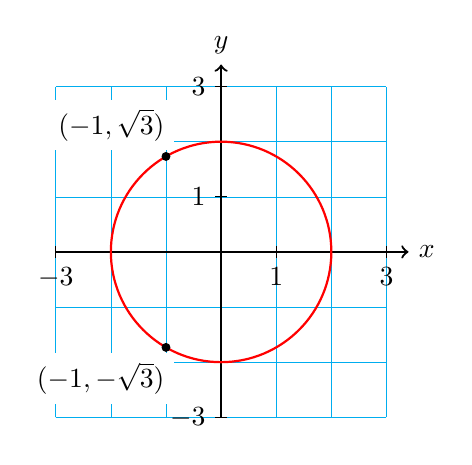
\begin{tikzpicture} [scale = .7]


\draw[step=1cm,cyan,very thin] (-3,-3) grid (3,3);
\draw[thick,->] (-3,0) -- (3.4,0) node[anchor=west] {$x$};
\draw[thick,->] (0,-3) -- (0,3.4) node[anchor=south] {$y$};
`
\foreach \x in {-3,1,3}
    \draw (\x cm,3pt) -- (\x cm,-3pt) node[anchor=north] {$\x$};
\foreach \y in {-3,1,3}
    \draw (3pt,\y cm) -- (-3pt,\y cm) node[anchor=east] {$\y$};


\coordinate(O) at (0,0);
\coordinate (A) at (-1,1.732 );
\coordinate (B) at (-1,-1.732 );

\draw[red,thick] (0,0) circle (2);

\filldraw[black] (A) circle (2pt) node[anchor=south east, xshift=3, yshift=2, fill=white]{\color{black}$(-1,\sqrt{3})$};
\filldraw[black] (B) circle (2pt) node[anchor=north east, xshift=3, yshift=-2, fill=white]{\color{black}$(-1,-\sqrt{3})$};

\end{tikzpicture}
\newline


exam1-3-4
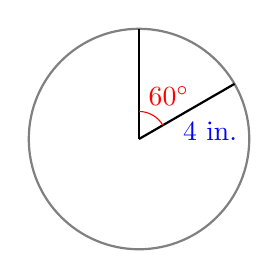
\begin{tikzpicture} [scale = .7]

\coordinate(O) at (0,0);
\coordinate (A) at (0,2 );
\coordinate (B) at (1.732,1 );

\draw[gray,thick] (0,0) circle (2);
\draw[black, thick] (O)--(B) node[below right, midway, xshift=-5] {\color{blue}4 in.};
\draw[black, thick] (O)--(A);
\draw[red, thin] (0,.5) arc (90:30:0.5) node[above right, midway, xshift=-5]{$60\degree$};


\end{tikzpicture}
\newline


hmwk 1.3.3
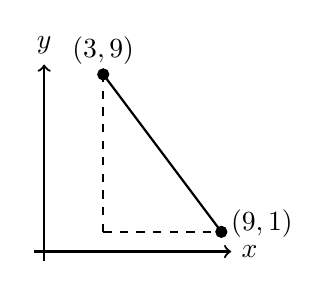
\begin{tikzpicture} [scale =0.25]

\coordinate(O) at (3,1);
\coordinate (A) at (3,9 );
\coordinate (B) at (9,1 );

\draw[black ,thick, ->] (-0.5,0) -- (9.5,0 ) node[anchor=west] {$x$};);
\draw[black ,thick, ->] (0,-0.5) -- (0,9.5 ) node[anchor=south] {$y$};);
\draw[black, thick, dashed] (O)--(B);
\draw[black, thick, dashed] (O)--(A);
\draw[black, thick] (B)--(A);

\filldraw[black] (A)  circle (8pt) node[anchor=south] {$(3,9)$};
\filldraw[black] (B)  circle (8pt) node[anchor=west, yshift=3] {$(9,1)$};

\end{tikzpicture}
\newline


hmwk 1.3.4
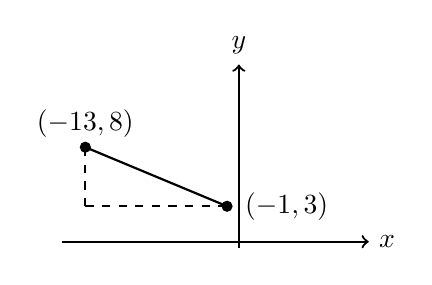
\begin{tikzpicture} [scale =0.15]

\coordinate(O) at (-13,3);
\coordinate (A) at (-13,8 );
\coordinate (B) at (-1,3 );

\draw[black ,thick, ->] (-15,0) -- (11,0 ) node[anchor=west] {$x$};);
\draw[black ,thick, ->] (0,-0.5) -- (0,15 ) node[anchor=south] {$y$};);
\draw[black, thick, dashed] (O)--(B);
\draw[black, thick, dashed] (O)--(A);
\draw[black, thick] (B)--(A);

\filldraw[black] (A)  circle (12pt) node[anchor=south] {$(-13,8)$};
\filldraw[black] (B)  circle (12pt) node[anchor=west, xshift=3] {$(-1,3)$};

\end{tikzpicture}
\newline


hmwk 1.3.5
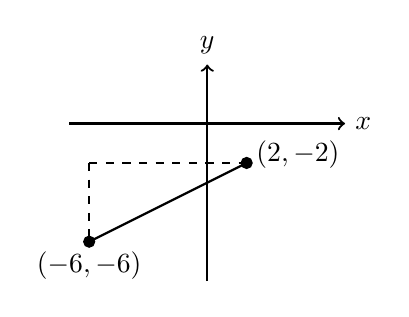
\begin{tikzpicture} [scale =0.25]

\coordinate(O) at (-6,-2);
\coordinate (A) at (-6,-6 );
\coordinate (B) at (2,-2 );

\draw[black ,thick, ->] (-7,0) -- (7,0 ) node[anchor=west] {$x$};);
\draw[black ,thick, ->] (0,-8) -- (0,3 ) node[anchor=south] {$y$};);
\draw[black, thick, dashed] (O)--(B);
\draw[black, thick, dashed] (O)--(A);
\draw[black, thick] (B)--(A);

\filldraw[black] (A)  circle (8pt) node[anchor=north] {$(-6,-6)$};
\filldraw[black] (B)  circle (8pt) node[anchor=west, yshift=3] {$(2,-2)$};


\end{tikzpicture}
\newline





hmwk 1.3.6
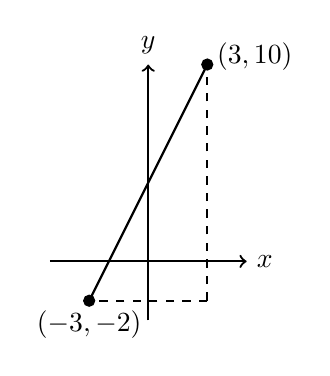
\begin{tikzpicture} [scale =0.25]

\coordinate(O) at (3,-2);
\coordinate (A) at (-3,-2 );
\coordinate (B) at (3,10 );

\draw[black ,thick, ->] (-5,0) -- (5,0 ) node[anchor=west] {$x$};);
\draw[black ,thick, ->] (0,-3) -- (0,10 ) node[anchor=south] {$y$};);
\draw[black, thick, dashed] (O)--(B);
\draw[black, thick, dashed] (O)--(A);
\draw[black, thick] (B)--(A);

\filldraw[black] (A)  circle (8pt) node[anchor=north] {$(-3,-2)$};
\filldraw[black] (B)  circle (8pt) node[anchor=west, yshift=3] {$(3,10)$};


\end{tikzpicture}
\newline

hmwk 1.3.13ans
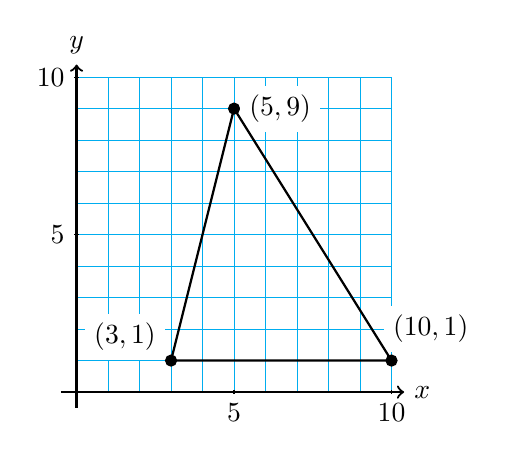
\begin{tikzpicture}[scale=.40]

\draw[step=1cm,cyan,very thin] (0,0) grid (10,10);
\draw[thick,->] (-.5,0) -- (10.4,0) node[anchor=west] {$x$};
\draw[thick,->] (0,-.5) -- (0,10.4) node[anchor=south] {$y$};
`
\foreach \x in {5,10}
    \draw (\x cm,2pt) -- (\x cm,-2pt) node[anchor=north] {$\x$};
\foreach \y in {5,10}
    \draw (2pt,\y cm) -- (-2pt,\y cm) node[anchor=east] {$\y$};


\coordinate (A) at (10,1);
\coordinate (B) at (3,1);
\coordinate (C) at (5,9);

\filldraw[black] (A) circle (5pt) node[anchor=south west, xshift=-3, yshift=3,fill=white] {$(10,1)$};
\filldraw[black] (B) circle (5pt) node[anchor=south east,xshift=-2,fill=white] {$(3,1)$};
\filldraw[black] (C) circle (5pt) node[anchor=west ,xshift=2,fill=white] {$(5,9)$};

\draw[black, thick] (A)--(C) -- (B) -- cycle;


\end{tikzpicture}
\newline

hmwk 1.3.25b
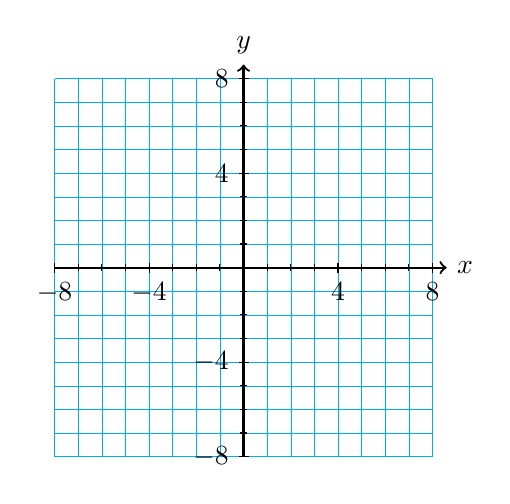
\begin{tikzpicture} [scale =0.3]

\draw[step=1cm,cyan,very thin] (-8,-8) grid (8,8);
\draw[thick,->] (-8,0) -- (8.6,0) node[anchor=west] {$x$};
\draw[thick,->] (0,-8) -- (0,8.6) node[anchor=south] {$y$};
`
\foreach \x in {-8,-4,4,8}
    \draw (\x cm,6pt) -- (\x cm,-6pt) node[anchor=north] {$\x$};
\foreach \y in {-8,-4,4,8}
    \draw (6pt,\y cm) -- (-6pt,\y cm) node[anchor=east] {$\y$};
\foreach \x in {-8,...,8}
    \draw (\x cm,4pt) -- (\x cm,-4pt) ;
\foreach \y in {-8,...,8}
    \draw (4pt,\y cm) -- (-4pt,\y cm) ;
\foreach \y in {-8,...,8}
    \draw (4pt,\y cm) -- (-4pt,\y cm) ;

\end{tikzpicture}
\newline

hmwk 1.3.25banswer
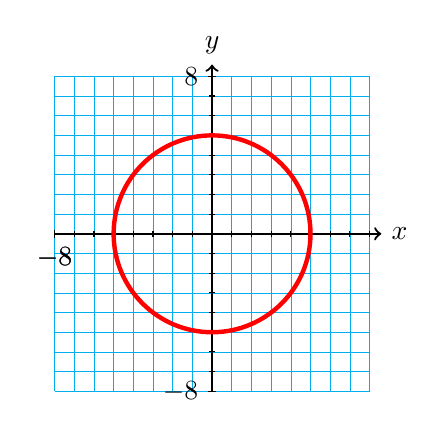
\begin{tikzpicture} [scale =0.25]

\draw[step=1cm,cyan,very thin] (-8,-8) grid (8,8);
\draw[thick,->] (-8,0) -- (8.6,0) node[anchor=west] {$x$};
\draw[thick,->] (0,-8) -- (0,8.6) node[anchor=south] {$y$};
`
\foreach \x in {-8,-8}
    \draw (\x cm,6pt) -- (\x cm,-6pt) node[anchor=north] {$\x$};
\foreach \y in {-8,8}
    \draw (6pt,\y cm) -- (-6pt,\y cm) node[anchor=east] {$\y$};
\foreach \x in {-8,...,8}
    \draw (\x cm,4pt) -- (\x cm,-4pt) ;
\foreach \y in {-8,...,8}
    \draw (4pt,\y cm) -- (-4pt,\y cm) ;
\foreach \y in {-8,...,8}
    \draw (4pt,\y cm) -- (-4pt,\y cm) ;

\draw[red, ultra thick] (0,0) circle (5cm);

\end{tikzpicture}
\newline


hmwk 1.3.26b
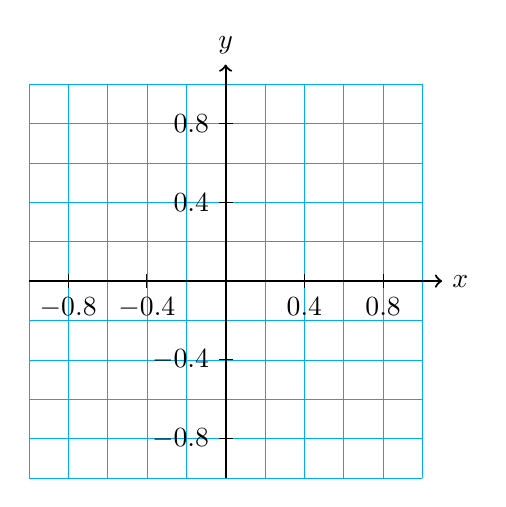
\begin{tikzpicture} [scale =2.5]

\draw[step=.2cm,cyan,very thin] (-1,-1) grid (1,1);
\draw[thick,->] (-1,0) -- (1.1,0) node[anchor=west] {$x$};
\draw[thick,->] (0,-1) -- (0,1.1) node[anchor=south] {$y$};
`
\foreach \x in {-0.8,-0.4, 0.4, 0.8}
    \draw (\x cm,1pt) -- (\x cm,-1pt) node[anchor=north] {$\x$};
\foreach \y in {-0.8,-0.4, 0.4, 0.8}
    \draw (1pt,\y cm) -- (-1pt,\y cm) node[anchor=east] {$\y$};

\end{tikzpicture}
\newline


hmwk 1.3.27answer
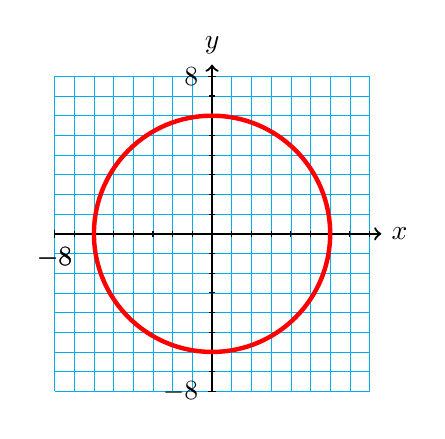
\begin{tikzpicture} [scale =0.25]

\draw[step=1cm,cyan,very thin] (-8,-8) grid (8,8);
\draw[thick,->] (-8,0) -- (8.6,0) node[anchor=west] {$x$};
\draw[thick,->] (0,-8) -- (0,8.6) node[anchor=south] {$y$};
`
\foreach \x in {-8,-8}
    \draw (\x cm,6pt) -- (\x cm,-6pt) node[anchor=north] {$\x$};
\foreach \y in {-8,8}
    \draw (6pt,\y cm) -- (-6pt,\y cm) node[anchor=east] {$\y$};
\foreach \x in {-8,...,8}
    \draw (\x cm,4pt) -- (\x cm,-4pt) ;
\foreach \y in {-8,...,8}
    \draw (4pt,\y cm) -- (-4pt,\y cm) ;
\foreach \y in {-8,...,8}
    \draw (4pt,\y cm) -- (-4pt,\y cm) ;

\draw[red, ultra thick] (0,0) circle (6cm);

\end{tikzpicture}
\newline


hmwk 1.3.29answer
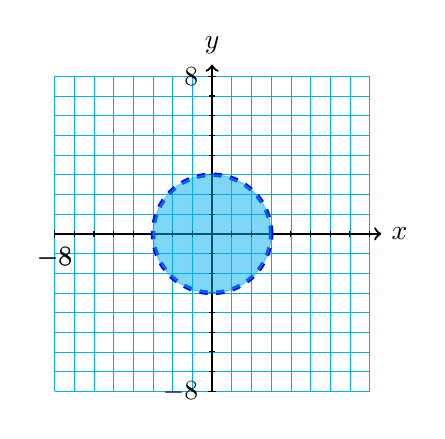
\begin{tikzpicture} [scale =0.25]

\draw[step=1cm,cyan,very thin] (-8,-8) grid (8,8);
\draw[thick,->] (-8,0) -- (8.6,0) node[anchor=west] {$x$};
\draw[thick,->] (0,-8) -- (0,8.6) node[anchor=south] {$y$};
`
\foreach \x in {-8,-8}
    \draw (\x cm,6pt) -- (\x cm,-6pt) node[anchor=north] {$\x$};
\foreach \y in {-8,8}
    \draw (6pt,\y cm) -- (-6pt,\y cm) node[anchor=east] {$\y$};
\foreach \x in {-8,...,8}
    \draw (\x cm,4pt) -- (\x cm,-4pt) ;
\foreach \y in {-8,...,8}
    \draw (4pt,\y cm) -- (-4pt,\y cm) ;
\foreach \y in {-8,...,8}
    \draw (4pt,\y cm) -- (-4pt,\y cm) ;

\draw[blue, ultra thick, dashed] (0,0) circle (3cm);
\filldraw[cyan, opacity=0.5] (0,0) circle (3cm);

\end{tikzpicture}
\newline

Hmwk 1.3.35-38 use an 8x8 grid, like 25b
Hmwk 35 has same answer as 27
\newline


hmwk 1.3.37answer
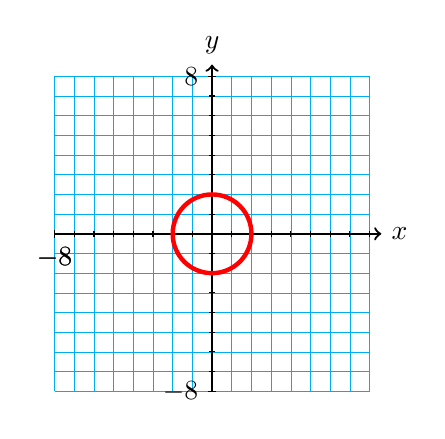
\begin{tikzpicture} [scale =0.25]

\draw[step=1cm,cyan,very thin] (-8,-8) grid (8,8);
\draw[thick,->] (-8,0) -- (8.6,0) node[anchor=west] {$x$};
\draw[thick,->] (0,-8) -- (0,8.6) node[anchor=south] {$y$};
`
\foreach \x in {-8,-8}
    \draw (\x cm,6pt) -- (\x cm,-6pt) node[anchor=north] {$\x$};
\foreach \y in {-8,8}
    \draw (6pt,\y cm) -- (-6pt,\y cm) node[anchor=east] {$\y$};
\foreach \x in {-8,...,8}
    \draw (\x cm,4pt) -- (\x cm,-4pt) ;
\foreach \y in {-8,...,8}
    \draw (4pt,\y cm) -- (-4pt,\y cm) ;
\foreach \y in {-8,...,8}
    \draw (4pt,\y cm) -- (-4pt,\y cm) ;

\draw[red, ultra thick] (0,0) circle (2cm);

\end{tikzpicture}
\newline


hmwk 1.3.39answer
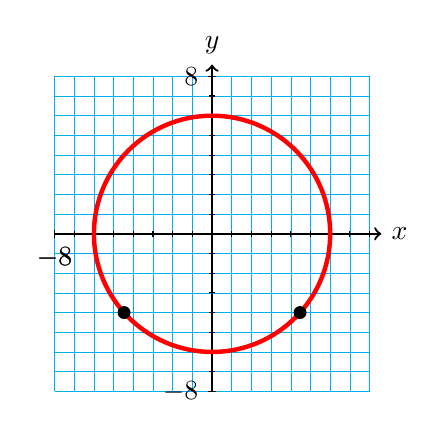
\begin{tikzpicture} [scale =0.25]

\draw[step=1cm,cyan,very thin] (-8,-8) grid (8,8);
\draw[thick,->] (-8,0) -- (8.6,0) node[anchor=west] {$x$};
\draw[thick,->] (0,-8) -- (0,8.6) node[anchor=south] {$y$};
`
\foreach \x in {-8,-8}
    \draw (\x cm,6pt) -- (\x cm,-6pt) node[anchor=north] {$\x$};
\foreach \y in {-8,8}
    \draw (6pt,\y cm) -- (-6pt,\y cm) node[anchor=east] {$\y$};
\foreach \x in {-8,...,8}
    \draw (\x cm,4pt) -- (\x cm,-4pt) ;
\foreach \y in {-8,...,8}
    \draw (4pt,\y cm) -- (-4pt,\y cm) ;
\foreach \y in {-8,...,8}
    \draw (4pt,\y cm) -- (-4pt,\y cm) ;

\draw[red, ultra thick] (0,0) circle (6cm);
\filldraw[black] (-4.47,-4) circle (0.3cm);
\filldraw[black] (4.47,-4) circle (0.3cm);

\end{tikzpicture}
\newline



Hmwk 1.3.41
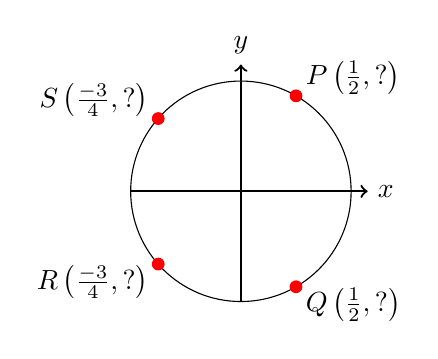
\begin{tikzpicture} [scale=0.7]

\coordinate(O) at (0,0);
\coordinate (P) at (1,1.732 );
\coordinate (Q) at (1,-1.732 );
\coordinate (R) at (-1.5,-1.32 );
\coordinate (S) at (-1.5,1.32);

\draw (0,0) circle (2);

\draw[thick,->] (-2,0) -- (2.3,0) node[anchor=west] {$x$};
\draw[thick,->] (0,-2) -- (0,2.3) node[anchor=south] {$y$};

\filldraw[red] (P) circle (3pt) node[anchor=south west, xshift=0, yshift=-3]{\color{black}$P\left(\frac{1}{2},? \right)$};
\filldraw[red] (Q) circle (3pt) node[anchor=north west, xshift=0, yshift=3]{\color{black}$Q\left(\frac{1}{2},? \right)$};
\filldraw[red] (R) circle (3pt) node[anchor=north east, xshift=0, yshift=3]{\color{black}$R\left(\frac{-3}{4},? \right)$};
\filldraw[red] (S) circle (3pt) node[anchor=south east, xshift=0, yshift=-3]{\color{black}$S\left(\frac{-3}{4},? \right)$};

\end{tikzpicture}
\newline



Hmwk 1.3.42
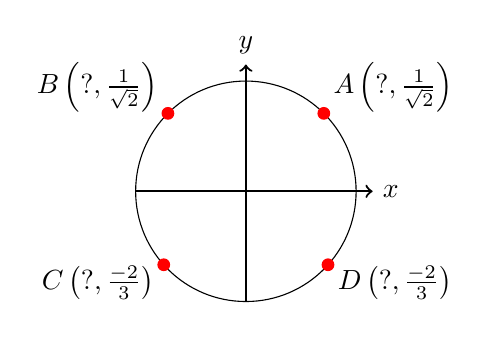
\begin{tikzpicture} [scale=0.7]

\coordinate(O) at (0,0);
\coordinate (A) at (1.414,1.414 );
\coordinate (D) at (1.49,-1.333 );
\coordinate (C) at (-1.49,-1.333 );
\coordinate (B) at (-1.414,1.414);

\draw (0,0) circle (2);

\draw[thick,->] (-2,0) -- (2.3,0) node[anchor=west] {$x$};
\draw[thick,->] (0,-2) -- (0,2.3) node[anchor=south] {$y$};

\filldraw[red] (A) circle (3pt) node[anchor=south west, xshift=0, yshift=-3]{\color{black}$A\left(?, \frac{1}{\sqrt{2}} \right)$};
\filldraw[red] (D) circle (3pt) node[anchor=north west, xshift=0, yshift=3]{\color{black}$D\left(?, \frac{-2}{3} \right)$};
\filldraw[red] (C) circle (3pt) node[anchor=north east, xshift=0, yshift=3]{\color{black}$C\left(?, \frac{-2}{3} \right)$};
\filldraw[red] (B) circle (3pt) node[anchor=south east, xshift=0, yshift=-3]{\color{black}$B\left(?, \frac{1}{\sqrt{2}} \right)$};

\end{tikzpicture}
\newline


Hmwk 1.3.43
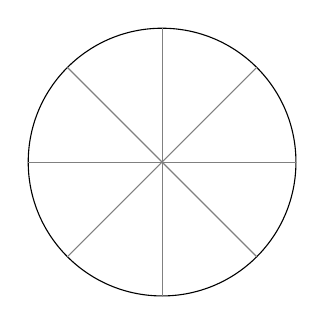
\begin{tikzpicture} [scale=0.85]

\coordinate(O) at (0,0);
\coordinate (A) at (1.414,1.414 );
\coordinate (B) at (1.414,-1.414 );
\coordinate (C) at (-1.414,-1.414 );
\coordinate (D) at (-1.414,1.414);

\draw (0,0) circle (2);

\draw[gray,thin] (A) --(C);
\draw[gray,thin] (B) --(D);
\draw[gray,thin] (-2,0) --(2,0);
\draw[gray,thin] (0,-2) --(0,2);

\end{tikzpicture}
\newline


Hmwk 1.3.45
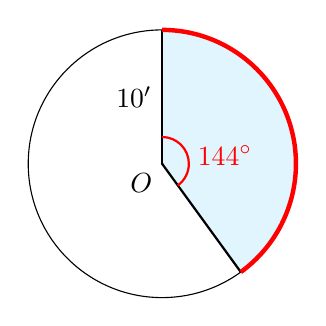
\begin{tikzpicture} [scale=0.85]

\coordinate(O) at (0,0);
\coordinate (A) at (1.176,-1.618 );
\coordinate (B) at (0,2 );

\filldraw[cyan!40!white!30] (A)--(O)--(B)--(B) arc (90:-54:2)--(A);
\draw (0,0) circle (2);

\draw[black,thick] (A) --(O);
\draw[black,thick] (B) --(O) node[left,midway] {$10'$};

\draw[red,thick] (0,.4) arc (90:-54:0.4) node[right, midway] {$144\degree$};
\draw[red, ultra thick] (B) arc (90:-54:2);
\filldraw[black] (O) circle (.2pt) node[anchor=north east] {$O$};

\end{tikzpicture}
\newline


Hmwk 1.3.46
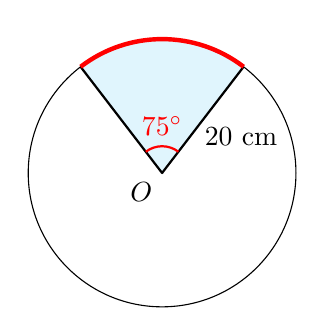
\begin{tikzpicture} [scale=0.85]

\coordinate(O) at (0,0);
\coordinate (A) at (1.218,1.587 );
\coordinate (B) at (-1.218,1.587 );

\filldraw[cyan!40!white!30] (B)--(O)--(A) arc (52.5:127.5:2)--(O);
\draw (0,0) circle (2);

\draw[black,thick] (A) --(O) node[right,midway,xshift=-3,yshift=-6] {$20$ cm};
\draw[black,thick] (B) --(O);

\draw[red,thick] (0.244,0.317) arc (52.5:127.5:0.4) node[above, midway] {$75\degree$};
\draw[red, ultra thick] (A) arc (52.5:127.5:2);
\filldraw[black] (O) circle (.2pt) node[anchor=north east] {$O$};

\end{tikzpicture}
\newline



Hmwk 1.3.47
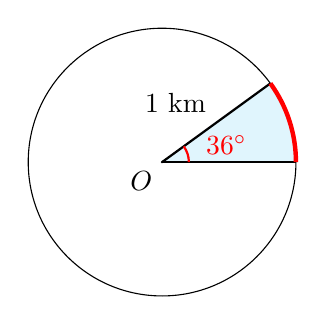
\begin{tikzpicture} [scale=0.85]

\coordinate(O) at (0,0);
\coordinate (A) at (2,0 );
\coordinate (B) at (1.618,1.176 );

\filldraw[cyan!40!white!30] (B)--(O)--(A) arc (0:36:2)--(O);
\draw (0,0) circle (2);

\draw[black,thick] (A) --(O);
\draw[black,thick] (B) --(O) node[above left,midway,xshift=0,yshift=0] {1 km};

\draw[red,thick] (0.4,0) arc (0:36:0.4) node[above right, midway,xshift=3, yshift=-4] {$36\degree$};
\draw[red, ultra thick] (A) arc (0:36:2);
\filldraw[black] (O) circle (.2pt) node[anchor=north east] {$O$};

\end{tikzpicture}
\newline



Hmwk 1.3.48
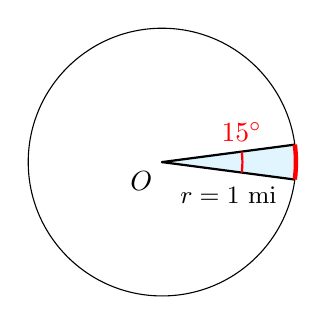
\begin{tikzpicture} [scale=0.85]

\coordinate(O) at (0,0);
\coordinate (A) at (1.983,-0.261 );
\coordinate (B) at (1.983, 0.261 );

\filldraw[cyan!40!white!30] (B)--(O)--(A) arc (-7.5:7.5:2)--(O);
\draw (0,0) circle (2);

\draw[black,thick] (A) --(O) node[below,midway,xshift=0,yshift=-2] {\small{$r=1$ mi}};
\draw[black,thick] (B) --(O);

\draw[red,thick] (1.19,-0.157) arc (-7.5:7.5:1.2) node[above , xshift=0, yshift=0] {$15\degree$};
\draw[red, ultra thick] (A) arc (-7.5:7.5:2);
\filldraw[black] (O) circle (.2pt) node[anchor=north east] {$O$};

\end{tikzpicture}
\newline


Hmwk 1.3.49
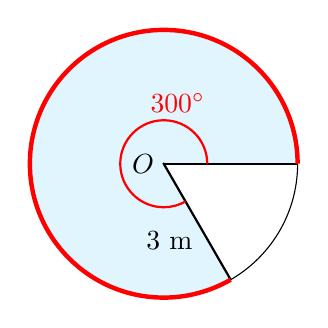
\begin{tikzpicture} [scale=0.85]

\coordinate(O) at (0,0);
\coordinate (A) at (2,0 );
\coordinate (B) at (1, -1.732 );

\filldraw[cyan!40!white!30] (B)--(O)--(A) arc (0:300:2)--(O);
\draw (0,0) circle (2);

\draw[black,thick] (A) --(O);
\draw[black,thick] (B) --(O) node[below left,midway,xshift=2,yshift=0] {$3$ m};

\draw[red,thick] (0.65,0) arc (0:300:.65) node[above , xshift=-.1cm, yshift=1.cm] {$300\degree$};
\draw[red, ultra thick] (A) arc (0:300:2);
\filldraw[black] (O) circle (.2pt) node[anchor= east] {$O$};

\end{tikzpicture}
\newline



Hmwk 1.3.50
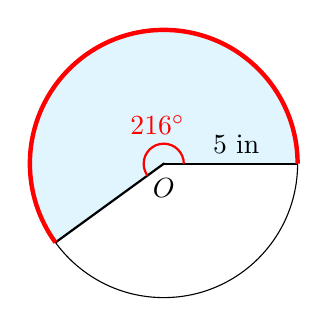
\begin{tikzpicture} [scale=0.85]

\coordinate(O) at (0,0);
\coordinate (A) at (2,0 );
\coordinate (B) at ( -1.618,-1.176 );

\filldraw[cyan!40!white!30] (B)--(O)--(A) arc (0:216:2)--(O);
\draw (0,0) circle (2);

\draw[black,thick] (A) --(O) node[above,midway,xshift=2,yshift=0] {$5$ in};
\draw[black,thick] (B) --(O);

\draw[red,thick] (0.3,0) arc (0:216:.3) node[above, midway, xshift=0, yshift=0] {$216\degree$};
\draw[red, ultra thick] (A) arc (0:216:2);
\filldraw[black] (O) circle (.2pt) node[anchor= north , yshift=-2] {$O$};

\end{tikzpicture}
\newline




Hmwk 1.3.51
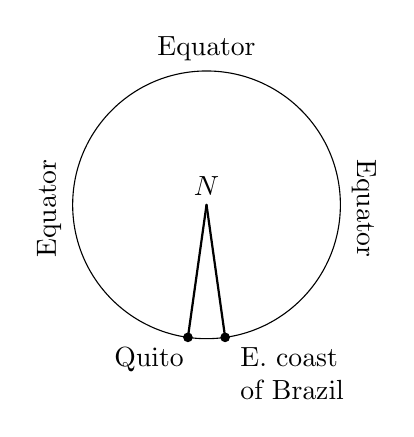
\begin{tikzpicture} [scale=0.85]

\coordinate(O) at (0,0);
\coordinate (A) at (0.278,-1.98 );
\coordinate (B) at (-0.278,-1.98 );

\draw (0,0) circle (2);

\draw[black,thick] (A) --(O) ;
\draw[black,thick] (B) --(O);

\filldraw[black] (O) circle (.2pt) node[anchor= south , xshift=0] {$N$};
\filldraw[black] (A) circle (1.8pt) node[anchor= north west, xshift=2,align=left] {E. coast \\of Brazil};
\filldraw[black] (B) circle (1.8pt) node[anchor= north east, xshift=2] {Quito};

\node[anchor = south] at (0,2) {Equator};
\node[anchor = west, xshift=.3cm, yshift=.7cm,rotate=-90] at (2,0) {Equator};
\node[anchor = east, xshift=-.3cm, yshift=.7cm, rotate=90] at (-2,0) {Equator};

\end{tikzpicture}
\newline



Hmwk 1.3.52
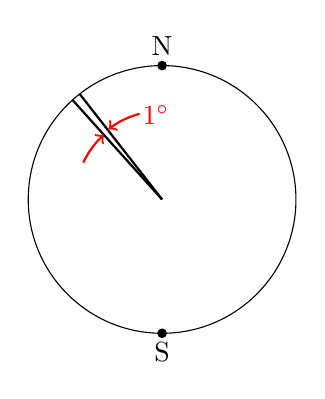
\begin{tikzpicture} [scale=0.85]

\coordinate(O) at (0,0);
\coordinate (A) at (-1.231,1.576 );
\coordinate (B) at (-1.338,1.486 );

\draw (0,0) circle (2);

\draw[black,thick] (A) --(O) ;
\draw[black,thick] (B) --(O);

\draw[red,thick, ->] (-.336,1.28) arc(105:128:1.3) node[above right,xshift=.3cm,yshift=-2] {$1\degree$};
\draw[red,thick, ->] (-1.178,0.549) arc(155:132:1.3) ;

\filldraw[black] (0,2) circle (1.8pt) node[anchor= south] {N};
\filldraw[black] (0,-2) circle (1.8pt) node[anchor= north , xshift=0] {S};

\end{tikzpicture}
\newline



Hmwk 1.3.53
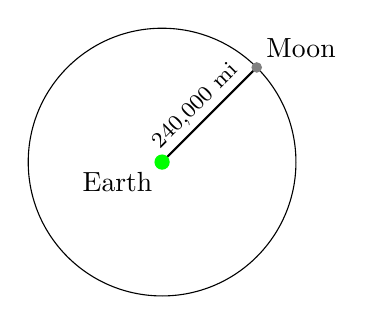
\begin{tikzpicture} [scale=0.85]

\coordinate(O) at (0,0);
\coordinate (A) at (1.414,1.414 );

\draw (0,0) circle (2);

\draw[black,thick] (A) --(O) node[above,midway,yshift=-2, rotate=45] {\footnotesize{240,000 mi}};


\filldraw[gray] (A) circle (2pt) node[anchor= south west] {\color{black}Moon};
\filldraw[green] (O) circle (3pt) node[anchor= north east, xshift=0] {\color{black}Earth};

\end{tikzpicture}
\newline



Hmwk 1.3.54
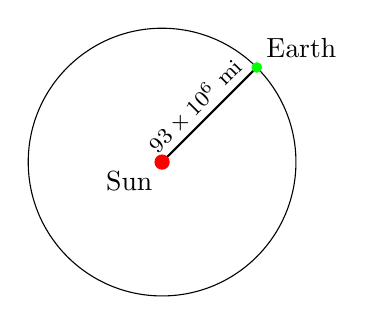
\begin{tikzpicture} [scale=0.85]

\coordinate(O) at (0,0);
\coordinate (A) at (1.414,1.414 );

\draw (0,0) circle (2);

\draw[black,thick] (A) --(O) node[above,midway,yshift=-2,rotate=45] {\footnotesize{$93\times 10^6$ mi}};


\filldraw[green] (A) circle (2pt) node[anchor= south west] {\color{black}Earth};
\filldraw[red] (O) circle (3pt) node[anchor= north east, xshift=0] {\color{black}Sun};

\end{tikzpicture}
\newline


Hmwk 1.3.56a
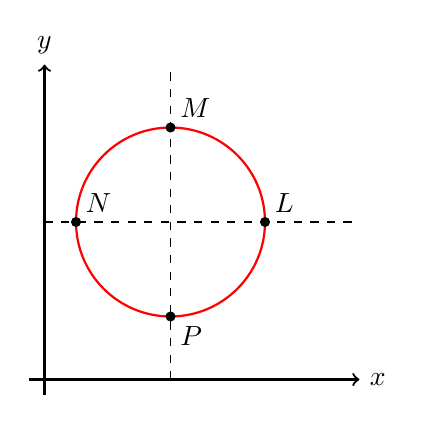
\begin{tikzpicture} [scale=0.4]

\coordinate(O) at (4,5);
\coordinate (L) at (7,5 );
\coordinate (M) at (4, 8);
\coordinate (N) at (1,5 );
\coordinate (P) at (4,2);

\draw[red,thick] (O) circle (3);

\draw[black,dashed] (0,5) --(10,5) ;
\draw[black,dashed] (4,0) --(4,10) ;
\draw[black,thick,->] (-.5,0) --(10,0) node[right] {$x$};
\draw[black,thick,->] (0,-0.5) --(0,10) node[above] {$y$};

\filldraw[black] (L) circle (4pt) node[anchor= south west] {\color{black}$L$};
\filldraw[black] (M) circle (4pt) node[anchor= south west] {\color{black}$M$};
\filldraw[black] (N) circle (4pt) node[anchor= south west] {\color{black}$N$};
\filldraw[black] (P) circle (4pt) node[anchor= north west] {\color{black}$P$};

\end{tikzpicture}
\newline


Hmwk 1.3.56b
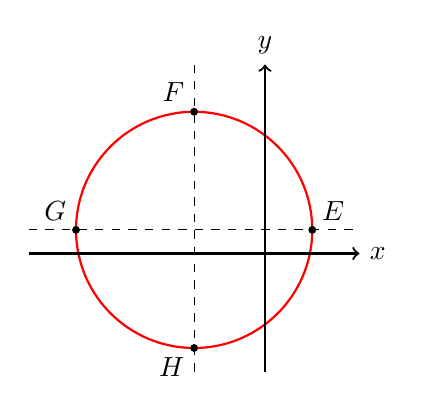
\begin{tikzpicture} [scale=0.3]

\coordinate(O) at (-3,1);
\coordinate (E) at (2,1 );
\coordinate (F) at (-3,6);
\coordinate (G) at (-8,1 );
\coordinate (H) at (-3,-4);

\draw[red,thick] (O) circle (5);

\draw[black,dashed] (-10,1) --(4,1) ;
\draw[black,dashed] (-3,-5) --(-3,8) ;
\draw[black,thick,->] (-10,0) --(4,0) node[right] {$x$};
\draw[black,thick,->] (0,-5) --(0,8) node[above] {$y$};

\filldraw[black] (E) circle (4pt) node[anchor= south west] {\color{black}$E$};
\filldraw[black] (F) circle (4pt) node[anchor= south east] {\color{black}$F$};
\filldraw[black] (G) circle (4pt) node[anchor= south east] {\color{black}$G$};
\filldraw[black] (H) circle (4pt) node[anchor= north east] {\color{black}$H$};

\end{tikzpicture}
\newline


Chap 1 review 5

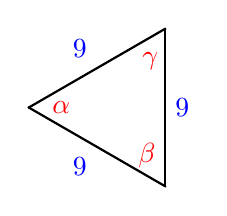
\begin{tikzpicture} 

\coordinate(A) at (0,0);
\coordinate (B) at (0,2 );
\coordinate (C) at (-1.732,1);

\draw[black,thick] (A)--(B) node[right,midway] {\color{blue}$9$};
\draw[black,thick] (A)--(C) node[below left,midway] {\color{blue}$9$};
\draw[black,thick] (C)--(B) node[above left,midway] {\color{blue}$9$};

\filldraw[black] (A) circle (.2pt) node[anchor= south east, xshift=0,yshift=3] {\color{red}$\beta$};
\filldraw[black] (B) circle (.2pt) node[anchor= north east,xshift=1,yshift=-5] {\color{red}$\gamma$};
\filldraw[black] (C) circle (.2pt) node[anchor= west,xshift=5] {\color{red}$\alpha$};

\end{tikzpicture}
\newline


Chap 1 review 6
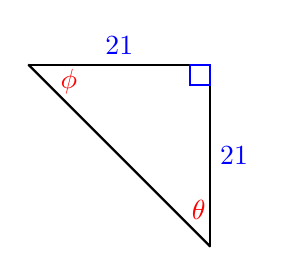
\begin{tikzpicture} 

\coordinate(A) at (0,0);
\coordinate (B) at (0,-2.3 );
\coordinate (C) at (-2.3,0);

\draw[black,thick] (A)--(B) node[right,midway] {\color{blue}$21$};
\draw[black,thick] (A)--(C) node[above,midway] {\color{blue}$21$};
\draw[black,thick] (C)--(B);

\draw[blue,thick] (A) rectangle +(-.25,-.25);
\filldraw[black] (B) circle (.2pt) node[anchor= south east,xshift=2,yshift=6] {\color{red}$\theta$};
\filldraw[black] (C) circle (.2pt) node[anchor= north west,xshift=8,yshift=2] {\color{red}$\phi$};

\end{tikzpicture}
\newline


Chap 1 review 7
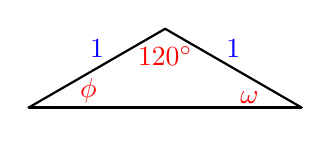
\begin{tikzpicture} 

\coordinate(A) at (0,0);
\coordinate (B) at (1.732,-1);
\coordinate (C) at (-1.732,-1);

\draw[black,thick] (A)--(B) node[above,midway] {\color{blue}$1$};
\draw[black,thick] (A)--(C) node[above,midway] {\color{blue}$1$};
\draw[black,thick] (C)--(B);

\filldraw[black] (A) circle (.2pt) node[anchor= north,xshift=0,yshift=-3] {\color{red}$120\degree$};
\filldraw[black] (B) circle (.2pt) node[anchor= south east,xshift=-12,yshift=-2] {\color{red}$\omega$};
\filldraw[black] (C) circle (.2pt) node[anchor= south west,xshift=15,yshift=-2] {\color{red}$\phi$};

\end{tikzpicture}
\newline


Chap 1 review 9
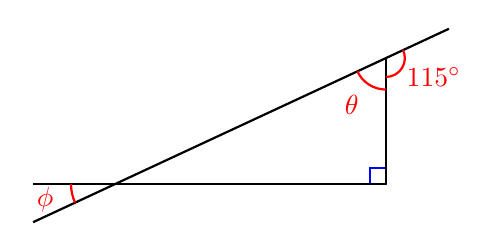
\begin{tikzpicture} [scale=0.8]

\coordinate (O) at (0,0);
\coordinate (y) at (0,2);
\coordinate (x) at (-4.3,0);

\draw[blue,  thick] (O) rectangle  +(-.25,.25)  ;
\draw[black,  thick] (-5.6,0) --  (O)  ;
\draw[black,  thick] (O) --  (y)   ;
\draw[black,  thick] (-5.6,-0.605) --  (1,2.465)  ;
\draw[red, thick] (0,1.7) arc (-90:{atan(2/4.3)}:.3) node [below right, midway,xshift=-2,yshift=4] {$115\degree$};
\draw[red, thick] (0,1.5) arc (-90:{atan(2/4.3)-180}:.5) node [below left, midway,xshift=0,yshift=0] {$\theta$};
\draw[red, thick] (-5,0) arc (180:{atan(2/4.3)+180}:0.7) node [below left, midway,xshift=-3,yshift=6] {$\phi$};

\end{tikzpicture}
\newline


Chap 1 review 10
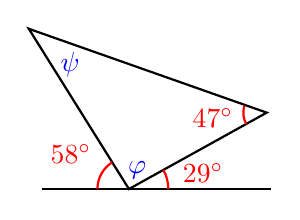
\begin{tikzpicture} [scale=1]

\coordinate (O) at (0,0);
\coordinate (A) at (1.75,0.97);
\coordinate (B) at (-1.272,2.035);

\filldraw (O) circle (.2pt) node[anchor=south, xshift=3] {\color{blue}$\varphi$};
\filldraw (B) circle (.2pt) node[anchor=north west, xshift=8,yshift=-5] {\color{blue}$\psi$};

\draw[black,  thick] (O) --  (A) --(B)--cycle  ;
\draw[black,  thick] (-1.1,0) --  (1.8,0)  ;
\draw[red, thick] (0.5,0) arc (0:29:.5) node [above right, midway,xshift=2,yshift=-5] {$29\degree$};
\draw[red, thick] (-.4,0) arc (180:122:.4) node [above left, midway,xshift=0,yshift=0] {$58\degree$};
\draw[red, thick] (1.49,0.824) arc (209:{180-atan(.935/3)}:.3) node [ left, midway,xshift=0,yshift=-1] {$47\degree$};

\end{tikzpicture}
\newline


Chap1rev11
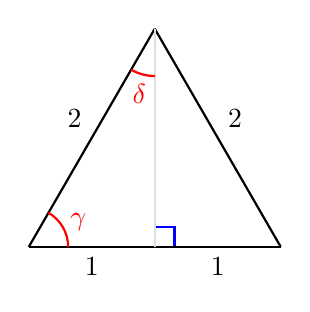
\begin{tikzpicture} [scale=1]

\coordinate (O) at (0,0);
\coordinate (A) at (3.2,0);
\coordinate (B) at (1.6,2.77);
\coordinate (C) at (1.6,0);

\draw[blue,thick] (C) rectangle +(0.25,0.25);
\draw[black,  thick] (O) --  (C) node[below,midway] {$1$}  ;
\draw[black,  thick] (A) --  (C) node[below,midway] {$1$}  ;
\draw[black,  thick] (O) --  (B) node[above left,midway] {$2$}  ;
\draw[black,  thick] (A) --  (B) node[above right,midway] {$2$}  ;
\draw[gray!50!white!50,  thick] (C) --  (B)  ;
\draw[red, thick] (0.5,0) arc (0:60:.5) node [above right, midway,xshift=-1,yshift=-5] {$\gamma$};
\draw[red, thick] (1.6,2.17) arc (-90:-120:.6) node [below left, midway,xshift=5,yshift=0] {$\delta$};

\end{tikzpicture}
\newline


Chap1rev12
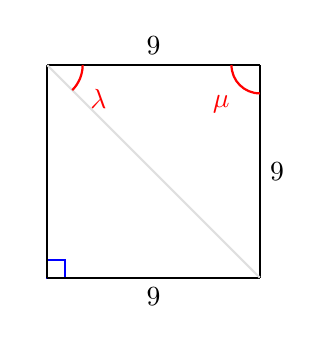
\begin{tikzpicture} [scale=.9]

\coordinate (O) at (0,0);
\coordinate (A) at (3,0);
\coordinate (B) at (3,3);
\coordinate (C) at (0,3);

\draw[blue,thick] (O) rectangle +(0.25,0.25);
\draw[black,  thick] (O) --  (A) node[below,midway] {$9$}  ;
\draw[black,  thick] (A) --  (B) node[right,midway] {$9$}  ;
\draw[black,  thick] (C) --  (B) node[ above,midway] {$9$}  ;
\draw[black,  thick] (C) --  (O) node[left,midway] {$$}  ;
\draw[gray!50!white!50,  thick] (C) --  (A)  ;
\draw[red, thick] (2.6,3) arc (180:270:.4) node [below left, midway,xshift=0,yshift=0] {$\mu$};
\draw[red, thick] (0.5,3) arc (0:-45:.5) node [below right, midway,xshift=0,yshift=0] {$\lambda$};

\end{tikzpicture}
\newline



Chap1rev13
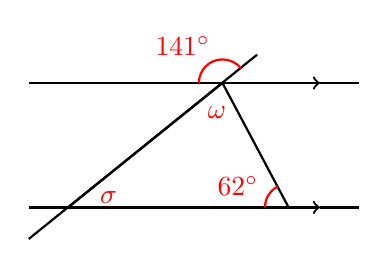
\begin{tikzpicture} [scale=1]

\coordinate (O) at (0,0);
\coordinate (A) at (2.8,0);
\coordinate (B) at (1.96,1.58);

\draw[black,  thick,->] (-.5,0) --  (3.2,0)  ;
\draw[black,  thick,->] (-.5,1.58) --  (3.2,1.58)  ;
\draw[black,  thick] (3.2,0) -- +(.5,0) ;
\draw[black,  thick] (3.2,1.58) -- +(.5,0)  ;
\draw[black,  thick] (-.5,-.4) --  (2.4,1.94)  ;
\draw[black,  thick] (A) --  (B)  ;
\draw[black,  thick] (O) --  (B)  ;
\draw[red, thick] (2.5,0) arc (180:118:.3) node [above left, midway,xshift=0,yshift=-4] {$62\degree$};
\draw[red, thick] (1.66,1.58) arc (180:39:.3) node [above left, midway, xshift=2,yshift=-2] {$141\degree$};
\filldraw[black] (O) circle (.2pt) node[anchor=south west,xshift=8,yshift=-2] {\color{red}$\sigma$};
\filldraw[black] (B) circle (.2pt) node[anchor=north,xshift=-2,yshift=-5] {\color{red}$\omega$};

\end{tikzpicture}
\newline



Chap1rev14
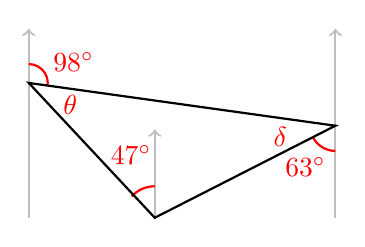
\begin{tikzpicture} [scale=.8]

\coordinate (O) at (0,0);
\coordinate (A) at (-2,2.14);
\coordinate (B) at (2.867,1.461);

\draw[gray!50!white,  thick,->] (-2,0) --  (-2,3)  ;
\draw[gray!50!white,  thick,->] (O) --  +(0,1.4)  ;
\draw[gray!50!white,  thick,->] (2.867,0) --  (2.867,3)  ;
\draw[red, thick] (-2,2.44) arc (90:-8:.3) node [above right, midway,xshift=0,yshift=-4] {$98\degree$};
\draw[red, thick] (2.867,1.061) arc (-90:-153:.4) node [below left, midway, xshift=5,yshift=0] {$63\degree$};
\draw[red, thick] (0,.5) arc (90:137:.5) node [above left, midway, xshift=7,yshift=5] {$47\degree$};
\filldraw[black] (A) circle (.2pt) node[anchor=north west,xshift=9,yshift=-1] {\color{red}$\theta$};
\filldraw[black] (B) circle (.2pt) node[anchor=east,xshift=-14,yshift=-4] {\color{red}$\delta$};
\draw[black,thick] (O)--(A)--(B)--cycle;

\end{tikzpicture}
\newline


Chap1rev15
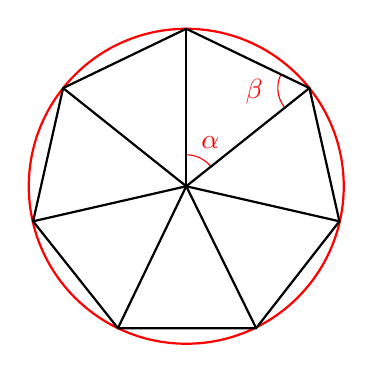
\begin{tikzpicture}
\coordinate(O) at (0,0);
\coordinate (A) at (0,2 );
\coordinate (B) at (1.564,1.247);
\coordinate (C) at(1.945,-0.445);
\coordinate (D) at (0.8878,-1.802);
\coordinate (E) at(-0.8678,-1.802);
\coordinate (F) at(-1.945,-0.445);
\coordinate (G) at(-1.564,1.247);

\draw[red,thick] (0,0) circle (2);
\draw[red] (0,0.4) arc(90:38.57:0.4) node[above right,midway, xshift=-3, yshift=0]{$\alpha$};
\draw[red] (1.25,0.998) arc(218.57:154.29:0.4) node[left, midway,xshift=-2, yshift=0]{$\beta$};

\draw[black,  thick] (A) -- (B) --( C) --(D) --(E)--(F) -- (G)--cycle;
\draw[black,  thick] (B) --  (O);
\draw[black,  thick] (C) --  (O);
\draw[black,  thick] (A)--(O);
\draw[black,  thick] (D) --  (O);
\draw[black,  thick] (E)--(O);
\draw[black,  thick] (F)--(O);
\draw[black,  thick] (G)--(O);

\end{tikzpicture}
\newline


Chap1rev16
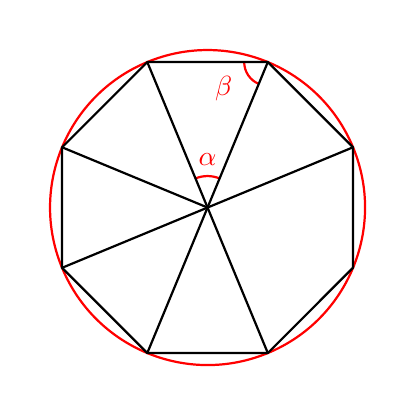
\begin{tikzpicture} [rotate=22.5]
\coordinate(O) at (0,0);
\coordinate (A) at (2,0 );
\coordinate (B) at (1.414,1.414);
\coordinate (C) at(0,2);
\coordinate (D) at (-1.414,1.414);
\coordinate (E) at(-2,0);
\coordinate (F) at(-1.414,-1.414);
\coordinate (G) at(0,-2);
\coordinate (H) at (1.414,-1.414);

\draw[red,thick] (0,0) circle (2);
\draw[red,thick] (0,0.4) arc(90:45:0.4) node[above,midway, xshift=0, yshift=0]{$\alpha$};
\draw[red,thick] (1.202,1.202) arc(225:157.5:0.3) node[left, midway,xshift=-2, yshift=-5]{$\beta$};

\draw[black,  thick] (A) -- (B) --( C) --(D) --(E)--(F) -- (G)--(H)--cycle;
\draw[black,  thick] (B) --  (O);
\draw[black,  thick] (C) --  (O);
\draw[black,  thick] (A)--(O);
\draw[black,  thick] (D) --  (O);
\draw[black,  thick] (E)--(O);
\draw[black,  thick] (F)--(O);
\draw[black,  thick] (G)--(O);

\end{tikzpicture}
\newline



Section 4.2 Angle of inclination
\begin{tikzpicture}

\coordinate (O) at (0,0);
\coordinate (x) at (3.5,0);
\coordinate (y) at (0,2);
\coordinate (A) at (3,1.8);
\coordinate (B) at (1.,0);
\coordinate (C) at (2.5,0);
\coordinate (D) at (-1,-1.8);

\draw[black,  thick, ->] (-1.5,0) --  (x) node[right] {$x$} ;
\draw[black,  thick, ->] (0,-2) --  (y) node[above] {$y$}  ;
\draw[black,  thick, <->] (D) --  (A)  ;
\draw[red, thick] (1.9,0) arc (0:{atan(0.9)}:.9) node [left, midway,xshift=0,yshift=-3] {$\alpha$};

\end{tikzpicture}
\newline

Section 4.2 Angle of inclination
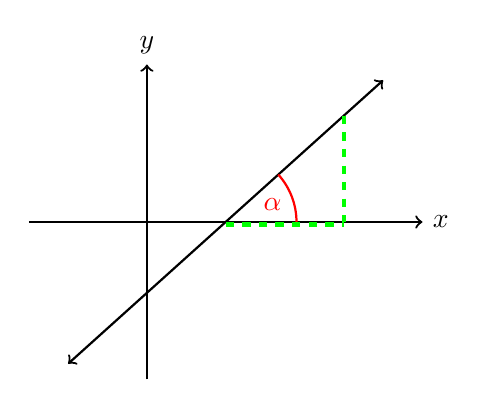
\begin{tikzpicture}

\coordinate (O) at (0,0);
\coordinate (x) at (3.5,0);
\coordinate (y) at (0,2);
\coordinate (A) at (3,1.8);
\coordinate (B) at (1.,0);
\coordinate (C) at (2.5,0);
\coordinate (D) at (-1,-1.8);

\draw[black,  thick, ->] (-1.5,0) --  (x) node[right] {$x$} ;
\draw[black,  thick, ->] (0,-2) --  (y) node[above] {$y$}  ;
\draw[black,  thick, <->] (D) --  (A)  ;
\draw[red, thick] (1.9,0) arc (0:{atan(0.9)}:.9) node [left, midway,xshift=0,yshift=-3] {$\alpha$};

\draw[green, ultra thick, dashed] (1,-.03) -- (2.5,-.03);
\draw[green, ultra thick, dashed] (2.5,1.35) -- (2.5,0);

\end{tikzpicture}
\newline


Exercise not used?
\begin{tikzpicture}
\coordinate (O) at (0,0);
\coordinate (A) at (0,0);
\coordinate (B) at (0,0);
\coordinate(C) at (0,0);
\coordinate (D) at (0,0);
\filldraw[black] (O) circle (.2pt) node[anchor=south west, xshift=6]{$50\degree$};
\filldraw[black] (A) circle (.2pt) node[anchor=south east]{$x$};
\filldraw[black] (B) circle (.2pt) node[anchor=north east, xshift=-6]{$y$};
\filldraw[black] (C) circle (.2pt) node[anchor=north west]{$z$};
%\draw[black,  thick] (A) -- (B) --( C) -- cycle;
\draw[black] (-2.3,0) --  (2.3,0);
\draw[black] (0.8,1.3) --  (-0.8,-1.3) ;
\end{tikzpicture}
\newline


\end{document}
